\documentclass{beamer}

\usepackage{geometry}
\usepackage{graphicx}
%\usepackage{wrapfig}
\usepackage{amsmath}

%\useoutertheme{infolines}
\usetheme{Boadilla}
\usecolortheme{seahorse}
\setbeamertemplate{navigation symbols}{}
\title{Data Structures}
\newcommand{\shorttitle}{64 Bit Intel Assembly Language}
\newcommand{\shortauthor}{\copyright 2011 Ray Seyfarth}
\author{Ray Seyfarth}
\begin{document}


\usefoottemplate{\vbox{
\tinycolouredline{structure!55}%
 {\color{white}{\textbf{\shorttitle}\hfill\textbf{\shortauthor}}}%
}}

\begin{frame}
    \titlepage
\end{frame}

\begin{frame}
    \frametitle{Data structures}
    \begin{itemize}
        \item Data structures can implement an ordering to data
        \begin{itemize}
            \item A stack where the items are ordered by time of insertion and
                  the newest item is removed first
            \item A queue where the items are ordered by time of insertion and
                  the oldest item is removed first
            \item A priority queue where items are ordered by priority
            \item A binary tree where items are kept in order based on a key
        \end{itemize}
        \item Some data structures implement a ``dictionary''
        \begin{itemize}
            \item Each item inserted has a ``key'', like a person's student id
            \item Information is stored with the key
            \item A hash table implements an efficient dictionary without maintaining
                  an ordering of keys
            \item A binary tree implements a dictionary keeping
                  the keys in order
        \end{itemize}
    \end{itemize}

\end{frame}

\begin{frame}
\frametitle{Outline}
\tableofcontents
\end{frame}

\section{Linked lists}

\begin{frame}[fragile]
    \frametitle{Linked lists}
    \begin{figure}[h!]
    \centering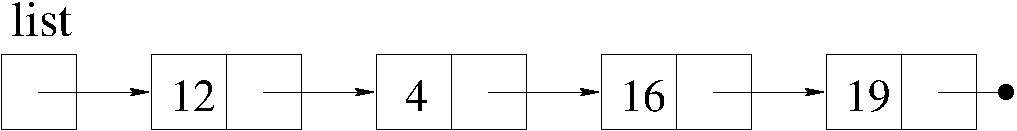
\includegraphics[width=4.0in]{linked_list_named.pdf}
    \end{figure}

    \begin{itemize}
        \item A simple linked list is constructed of a sequence of structs
        \item Each struct has some data and a pointer to the next item on the list
        \item The filled circle means a pointer equal to NULL (0)
        \item There needs to be some memory cell containing the first pointer
        \item This list has no obvious order to the keys
        \item It could be ordered by insertion time in two ways: by inserting
              at the front or the end
        \item It is easier to insert at the front, though the value of {\tt list}
              will change with each insertion
    \end{itemize}

\end{frame}

\begin{frame}[fragile]
    \frametitle{List node struct definition}
\begin{verbatim}
        struc   node
n_value resq    1
n_next  resq    1
        align   8
        endstruc
\end{verbatim}
    \begin{itemize}
        \item Using ``{\tt align 8}'' insures that the size is a multiple
              of 8 bytes
        \item This is not needed here since, both {\tt node} items are quad words
        \item It's ``defensive programming'' to insert it now in case the 
              definition changes
    \end{itemize}
\end{frame}

\begin{frame}[fragile]
    \frametitle{Creating an empty list}
    \begin{itemize}
        \item The only requirement will be to set the pointer to NULL
        \item Having a function makes it possible to change later with
              less impact on the rest of the program
    \end{itemize}

\begin{verbatim}
newlist:
        xor     eax, eax
        ret
        ...
        call    newlist
        mov     [list], rax
\end{verbatim}
\end{frame}

\begin{frame}[fragile]
    \frametitle{Inserting a number into a list}
    \begin{itemize}
        \item A new {\tt node} will be allocated and placed at the start
        \item We must pass the list pointer into the function
        \item We also must receive a new pointer back to store in {\tt list}
        \item In C we would use
    \end{itemize}
\begin{verbatim}
    list = insert ( list, k );
\end{verbatim}    
    \begin{itemize}
        \item In assembly we would insert k using
    \end{itemize}
\begin{verbatim}
    mov     rdi, [list] ; pass in the list pointer
    mov     rsi, [k]
    call    insert
    mov     [list], rax ; we have a new list pointer
\end{verbatim}
\end{frame}

\begin{frame}[fragile]
    \frametitle{Insert code}
\begin{verbatim}
insert:
.list   equ     0
.k      equ     8
        push    rbp
        mov     rbp, rsp
        sub     rsp, 16
        mov     [rsp+.list], rdi  ; save list pointer
        mov     [rsp+.k], rsi     ; and k on stack
        mov     edi, node_size
        call    malloc            ; rax will be node pointer
        mov     r8, [rsp+.list]   ; get list pointer
        mov     [rax+n_next], r8  ; save pointer in node
        mov     r9, [rsp+.k]      ; get k
        mov     [rax+n_value], r9 ; save k in node
        leave
        ret
\end{verbatim}    
\end{frame}

\begin{frame}[fragile]
    \frametitle{Traversing the list}
\footnotesize
\begin{verbatim}
print:
        push    rbp
        mov     rbp, rsp
        sub     rsp, 16           ; subtract multiples of 16
        mov     [rsp], rbx        ; save old value of rbx
        cmp     rdi, 0
        je      .done
        mov     rbx, rdi
.more   lea     rdi, [.print_fmt]
        mov     rsi, [rbx+n_value]
        xor     eax, eax
        call    printf
        mov     rbx, [rbx+n_next]
        cmp     rbx, 0
        jne     .more
.done   lea     rdi, [.newline]
        xor     eax, eax
        call    printf
        mov     rbx, [rsp]        ; restore rbx
        leave
        ret
\end{verbatim}
\end{frame}

\begin{frame}[fragile]
    \frametitle{Main program to build a list}
\footnotesize
\begin{verbatim}
main:
        push    rbp
        mov     rbp, rsp
        sub     rsp, 16
        call    newlist
        mov     [rsp+.list], rax  ; .list equal to 0, not shown
.more   lea     rdi, [.scanf_fmt] ; .scanf_fmt not shown
        lea     rsi, [rsp+.k]     ; .k equal to 8, not shown
        xor     eax, eax          ; no floating point value parameters
        call    scanf
        cmp     rax, 1            ; quit it scanf does not return 1
        jne     .done
        mov     rdi, [rsp+.list]  ; Get the list pointer
        mov     rsi, [rsp+.k]     ; Get k
        call    insert
        mov     [rsp+.list], rax  ; Save new list pointer
        mov     rdi, rax          ; Move the pointer to be a parameter
        call    print
        jmp     .more             ; Try to read another number
.done   leave
        ret
\end{verbatim}
\end{frame}

\section{Doubly linked lists}

\begin{frame}[fragile]
    \frametitle{Doubly linked lists}
\begin{figure}[h!]
\centering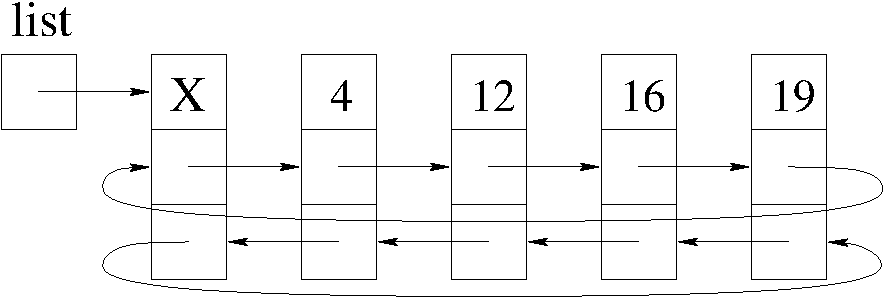
\includegraphics[width=3.5in]{doubly_linked_list.pdf}
\end{figure}
    \begin{itemize}
        \item This list uses forwards and backwards pointers to make a cycle
        \item Also the first node is not used, so an empty list
              will have one node and will be circular
        \item The first node is called a ``head'' node
        \item Using a head node and a circular list makes insertion trivial
        \item You can also insert and remove from either end easily
    \end{itemize}
\end{frame}


\begin{frame}[fragile]
    \frametitle{Doubly linked list {\tt node} struct}
\begin{verbatim}
            struc   node
    n_value resq    1
    n_next  resq    1
    n_prev  resq    1
            align   8
            endstruc
\end{verbatim}
    \begin{itemize}
        \item An ``empty'' list is still circular
        \item There are no special cases to consider
    \end{itemize}
\begin{center}
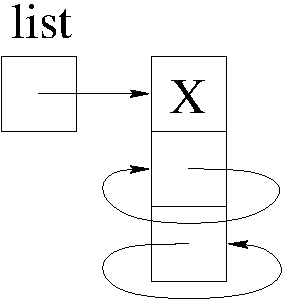
\includegraphics[width=1.0in]{empty_doubly_linked_list.pdf}
\end{center}
\end{frame}

\begin{frame}[fragile]
    \frametitle{Inserting at the front of a doubly linked list}
\begin{center}
\centering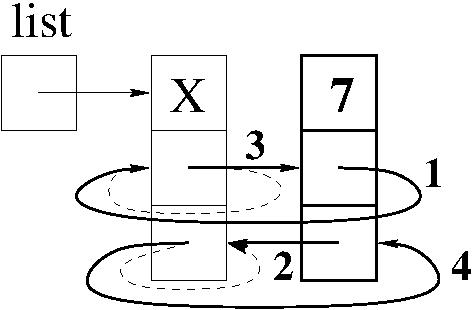
\includegraphics[width=1.5in]{insert_doubly_linked_list.pdf}
\end{center}
    \begin{itemize}
        \item The original links are dashed lines
        \item Make the new node point forward to the head cell's next
        \item Make the new node point backward to the head cell
        \item Make the head cell point forward to the new cell
        \item Make the new cell's next node point backward to the new cell
    \end{itemize}
\end{frame}

\begin{frame}[fragile]
    \frametitle{Insertion function}
\small
\begin{verbatim}
;       insert ( list, k );
insert: push    rbp
        mov     rbp, rsp
        sub     rsp, 16
        mov     [rsp+.list], rdi  ; save list pointer, .list equ 0
        mov     [rsp+.k], rsi     ; and k on stack, .k equ 8
        mov     edi, node_size
        call    malloc            ; rax will be node pointer
        mov     r8, [rsp+.list]   ; get list pointer
        mov     r9, [r8+n_next]   ; get head's next
        mov     [rax+n_next], r9  ; set new node's next
        mov     [rax+n_prev], r8  ; set new node's prev
        mov     [r8+n_next], rax  ; set head's next
        mov     [r9+n_prev], rax  ; set new node's next's prev
        mov     r9, [rsp+.k]      ; get k
        mov     [rax+n_value], r9 ; save k in node
        leave
        ret
\end{verbatim}
\end{frame}

\begin{frame}[fragile]
    \frametitle{List traversal}
\footnotesize
\begin{verbatim}
;       print ( list );
print:  push    rbp
        mov     rbp, rsp
        sub     rsp, 16
        mov     [rsp+.rbx], rbx   ; save rbx, .rbx equ 0
        mov     [rsp+.list], rdi  ; save list, .list equ 8
        mov     rbx, [rdi+n_next] ; skip the nead node
        cmp     rbx, [rsp+.list]  ; is the list empty?
        je      .done
.more   lea     rdi, [.print_fmt] ; .print_fmt not shown
        mov     rsi, [rbx+n_value]
        call    printf            ; print the node's value
        mov     rbx, [rbx+n_next] ; advance to the next node
        cmp     rbx, [rsp+.list]  ; have we reached the head cell?
        jne     .more
.done   lea     rdi, [.newline]   ; .newline not shown
        call    printf
        mov     rbx, [rsp+.rbx]   ; restore rbx
        leave
        ret
\end{verbatim}
\end{frame}

\section{Hash tables}

\begin{frame}
    \frametitle{Hash tables}
    \begin{itemize}
        \item For each key, compute a hash value
        \item The hash value defines an index in an array to store the key
        \item Collisions occur when 2 different keys hash to the same index
        \item The simplest collision resolution is to use a linked list
    \end{itemize}
\begin{center}
\centering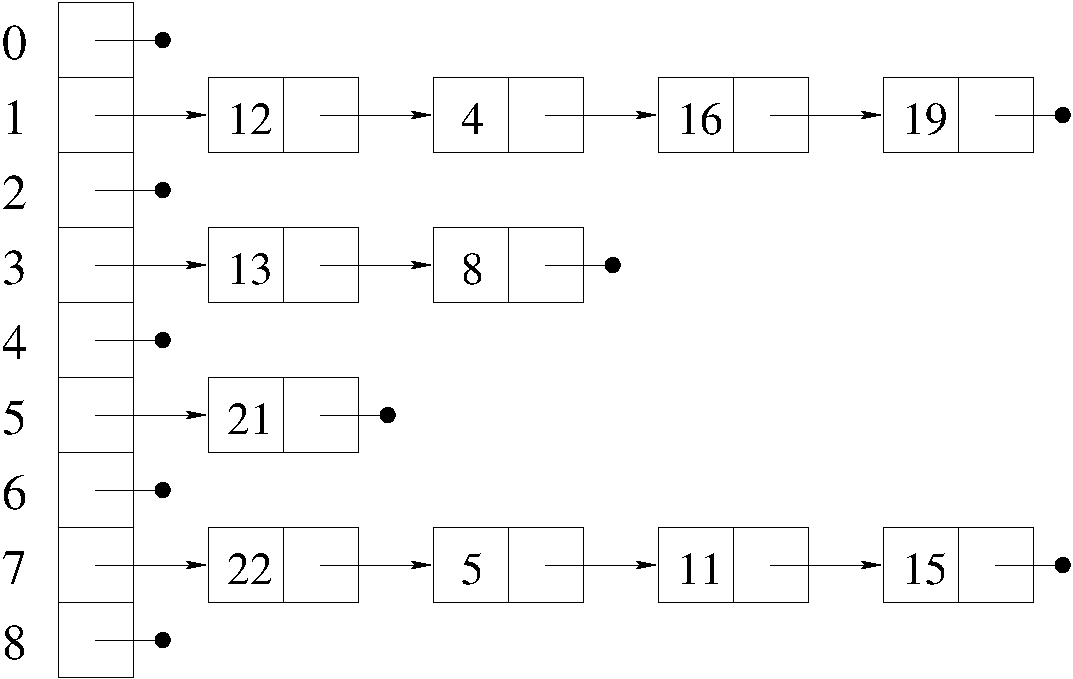
\includegraphics[width=3.2in]{hash_table.pdf}
\end{center}
\end{frame}

\begin{frame}[fragile]
    \frametitle{A good hash function for integers}
    \begin{itemize}
        \item A good hash function spreads the keys around
        \item Using $k \mod t$ where $t$ is the table size is good
        \item It could be bad if the keys are related to the table size
        \item A good recommendation is to make $t$ prime
        \item In this example, $t=256$, so using {\tt and} works
    \end{itemize}

\begin{verbatim}
;       i = hash ( n );
hash    mov     rax, rdi
        and     rax, 0xff
        ret
\end{verbatim}
\end{frame}

\begin{frame}[fragile]
    \frametitle{A good hash function for strings}
    \begin{itemize}
        \item The code below uses the characters of the string as
              coefficients of a polynomial
        \item The polynomial is evaluated at 191 (a prime)
        \item Then a mod is done with 100000 to get the hash value
        \item Assembly code is an exercise for the reader
    \end{itemize}

\begin{verbatim}
    int hash ( unsigned char *s )
    {
        unsigned long h = 0;
        int i = 0;
        
        while ( s[i] ) {
            h = h*191 + s[i];
            i++;
        }
        return h % 100000;
    }
\end{verbatim}
\end{frame}


\begin{frame}[fragile]
    \frametitle{Hash node structure and array of pointers}
    \begin{itemize}
        \item The hash table has only 256 pointers
        \item Usually the array would be larger and a creation function needed
    \end{itemize}

\begin{verbatim}
        segment .data
table   times 256 dq    0   ; All NULL pointers
        struc  node
n_value resq    1
n_next  resq    1           ; Singly linked list
        align   8
        endstruc
\end{verbatim}
\end{frame}

\begin{frame}[fragile]
    \frametitle{Function to find a key}
\small
\begin{verbatim}
;       p = find ( n );
;       p = 0 if not found
find:   push    rbp
        mov     rbp, rsp
        sub     rsp, 16
        mov     [rsp], rdi         ; save key
        call    hash
        mov     rax, [table+rax*8] ; get pointer
        mov     rdi, [rsp]         ; get key
        cmp     rax, 0             ; empty list?
        je      .done
.more   cmp     rdi, [rax+n_value] ; key match?
        je      .done
        mov     rax, [rax+n_next]  ; advance on the collision list
        cmp     rax, 0             ; end of list
        jne     .more
.done   leave
        ret
\end{verbatim}
\end{frame}

\begin{frame}[fragile]
    \frametitle{Function to insert a key}
\small
\begin{verbatim}
insert: push    rbp
        mov     rbp, rsp
        sub     rsp, 16
        mov     [rsp+.n], rdi     ; save n, .n equ 0
        call    find
        cmp     rax, 0            ; Is n already there?
        jne     .found
        mov     rdi, [rsp+.n]     ; compute hash(n)
        call    hash
        mov     [rsp+.h], rax     ; save hash value
        mov     rdi, node_size    ; allocate a node
        call    malloc
        mov     r9, [rsp+.h]      ; use r9 as index register
        mov     r8, [table+r9*8]  ; get old pointer from table
        mov     [rax+n_next], r8  ; make new node point to old
        mov     r8, [rsp+.n]      ; get n from the stack
        mov     [rax+n_value], r8 ; set the node value
        mov     [table+r9*8], rax ; make new node first on its list
.found  leave
        ret
\end{verbatim}
\end{frame}

\begin{frame}
    \frametitle{Testing the hash table}
    \begin{itemize}
        \item Need to examine print function
        \item Need to examine main function
        \item Test the program
    \end{itemize}
\end{frame}

\section{Binary trees}

\begin{frame}[fragile]
    \frametitle{Binary trees}
    \begin{itemize}
        \item A binary tree is a hierarchy of nodes
        \item There is a root node (or not, for an empty tree)
        \item Each node can have a left child and a right child
        \item The node structure has 2 pointers
        \item Either or both pointers could be NULL
        \item Binary trees are usually ordered like having all keys less
              the current key in the left subtree
        \item Such a tree is a ``binary search tree''
    \end{itemize}
\begin{verbatim}
        struc   node
n_value resq    1
n_left  resq    1
n_right resq    1
        align   8
        endstruc
\end{verbatim}
\end{frame}

\begin{frame}[fragile]
    \frametitle{A structure for the tree}
    \begin{itemize}
        \item We could represent an empty tree as a NULL pointer
        \item This introduces special cases
        \item Instead we implement a {\tt tree} struct
        \item It contains the root pointer which can be NULL
        \item It also contains the count of nodes in the tree
        \item After creating a tree, we use the same pointer
              for all function calls
    \end{itemize}

\begin{verbatim}
        struc   tree
t_count resq    1
t_root  resq    1
        align   8
        endstruc
\end{verbatim}
\end{frame}

\begin{frame}[fragile]
    \frametitle{Creating a new tree}
    \begin{itemize}
        \item The {\tt new\_tree} function allocates a {\tt tree}
              struct and sets it up as an empty tree
    \end{itemize}
\begin{verbatim}
new_tree:
        push    rbp
        mov     rbp, rsp
        mov     rdi, tree_size
        call    malloc
        xor     edi, edi
        mov     [rax+t_root], rdi
        mov     [rax+t_count], rdi
        leave
        ret
\end{verbatim}
\end{frame}

\begin{frame}[fragile]
    \frametitle{Finding a node in a tree: p = find(t,n)}
\small
\begin{verbatim}
find:   push    rbp
        mov     rbp, rsp
        mov     rdi, [rdi+t_root]
        xor     eax, eax
.more   cmp     rdi, 0
        je      .done
        cmp     rsi, [rdi+n_value]
        jl      .goleft
        jg      .goright
        mov     rax, rsi
        jmp     .done
.goleft:
        mov     rdi, [rdi+n_left]
        jmp     .more
.goright:
        mov     rdi, [rdi+n_right]
        jmp     .more
.done   leave
        ret
\end{verbatim}
\end{frame}

\begin{frame}
    \frametitle{Inserting a node into a tree}
    \begin{itemize}
        \item The code is too long for a slide
        \item First you check to see if the key is already in the tree
        \item If not, then you create a new node and set it value and
              set its two kids to NULL
        \item There is a special case for an empty tree
        \item If not empty, then we must traverse down the tree, going
              sometimes left and sometimes right to find the right place
              to insert the new node
    \end{itemize}
\end{frame}

\begin{frame}[fragile]
    \frametitle{Printing the keys in order}
    \begin{itemize}
        \item We first call a non-recursive function with the tree object
        \item It calls a recursive function with the root node
    \end{itemize}
\begin{verbatim}
;       print(t);
print:
        push    rbp
        mov     rbp, rsp
        mov     rdi, [rdi+t_root]
        call    rec_print
        segment .data
.print  db      0x0a, 0
        segment .text
        lea     rdi, [.print]
        call    printf
        leave
        ret
\end{verbatim}
\end{frame}

\begin{frame}[fragile]
    \frametitle{Recursive print function: rec\_print(t)}
\small
\begin{verbatim}
rec_print: push    rbp
           mov     rbp, rsp
           sub     rsp, 16           ; make room to save t
           cmp     rdi, 0            ; return if t is NULL
           je      .done
           mov     [rsp+.t], rdi     ; save t, .t equ 0
           mov     rdi, [rdi+n_left] ; print the left sub-tree
           call    rec_print
           mov     rdi, [rsp+.t]     ; print the current node
           mov     rsi, [rdi+n_value]
           lea     rdi, [.print]     ; .print: format string
           call    printf
           mov     rdi, [rsp+.t]     ; print the right sub-tree
           mov     rdi, [rdi+n_right]
           call    rec_print
.done      leave
           ret
\end{verbatim}
\end{frame}

\end{document}
